\documentclass[11pt]{article}
\usepackage[margin=1in]{geometry}
\usepackage[T1]{fontenc}
\usepackage{lmodern}
\usepackage{microtype}
\usepackage{graphicx}
\usepackage{booktabs}
\usepackage{amsmath}
\usepackage[hidelinks]{hyperref}
\usepackage{url}

\title{The .300 hitter after 2008: a pre-registered held-out test of the round-number claims of Pope and Simonsohn}
\author{Qianghao Wu}
\date{28 November 2026}

\begin{document}
\maketitle

\begin{abstract}
Pope and Simonsohn (2011) reported that Major League Baseball batters of 1975--2008 were nearly 4 times as likely to end a season at a .300 batting average as at .299. They also reported that in the last scheduled plate appearance of the season, batters at .299 never walked (0 of 61), got more hits, and were rarely replaced by a pinch hitter, while batters at .300 were often replaced. We re-tested these statements on the seasons 2009--2025, which were not in the original sample, with a protocol that we committed before we computed any outcome. The data are the public Retrosheet event files. Our parsed season totals agree with the MLB Stats API for 5,446 of 5,447 batter-seasons with at least 200 at-bats. The season-end excess at .300 is a re-test: three earlier studies re-tested it, and one already reports a smaller ratio for 2005--2018. The excess persists: 47 batter-seasons end at .300 and 20 at .299 (ratio 2.35, 95\% CI 1.37--4.19; one-sided binomial $p = 0.00065$). The pre-registered rule also required the .300 ratio to exceed the ratio at 10 placebo thresholds, and it did not (.330: 8 vs 3). So this claim is not supported under the registered rule. The final-plate-appearance statements had no held-out test before. The zero count of walks at .299 does not persist (3 walks in 23 plate appearances), and we find no walk suppression ($p = 0.89$). The hit advantage at .299 has the paper's direction but is not significant (.421 vs .200, $p = 0.125$). In a post hoc, exploratory analysis with the paper's own definitions, the substitution pattern is present: a pinch hitter took 30.0\% of the last scheduled plate appearances at .300 and 5.7\% at the other values from .280 to .320 (Holm-adjusted $p = 0.0002$). The post hoc substitution result and the descriptive exit check agree better with batters who stop at .300 than with batters who hit better below it. This work has not yet been reviewed by experts. The computations and the text were produced by AI models (from Anthropic and OpenAI), working under the author's direction.
\end{abstract}

\section{Introduction}

A round number can act as a goal. Pope and Simonsohn \cite{ps2011} gave baseball as their first field example. In Retrosheet play-by-play data for 1975--2008, among batters with at least 200 at-bats (8,817 player-seasons), 1.40\% ended the season at .300 and 0.38\% at .299. In their words, ``professional batters are nearly 4 times as likely to end the season with a .300 batting average as they are to end the season with a .299 average'' \cite[Study 1]{ps2011}. They then looked at the last scheduled plate appearance (PA) of the season. Batters at .298 or .299 got a hit in 35.2\% of these PAs, against 22.4\% at .300 or .301. At .299 the share was 43\%, against 22.8\% at the other values from .280 to .320. Batters at .298 or .299 walked in 2.5\% of these PAs, against 8.6\% at .300 or .301, and ``not a single player (out of 61) walked when his season average was .299'' \cite[Study 1]{ps2011}. A pinch hitter replaced the batter in 4.1\% of these PAs at .298 or .299 and in 19.7\% at .300 or .301; at .300 alone the share was 34.3\%, against 7.0\% for all the players in their figure. The denominator of each share includes outs, hits, walks and substitutions \cite[note 4]{ps2011}. The authors themselves wrote that the high hit share at .299 ``is likely to be at least partially explained by batters ending their season prematurely'' \cite[Study 1]{ps2011}.

Scott and Birnbaum \cite{sb2010} challenged the hit result. They used all PAs in the team's last two games, so that the sample does not depend on which PA was the last. Batters for whom a hit would reach .300 hit .299 (155 for 517). Batters at .300 or more for whom an out would drop the average below .300 hit .297 (43 for 145). They concluded that ``sampling bias fully accounts for Pope and Simonsohn's findings.''

Three later studies re-tested the season-end excess. Tanji \cite{tanji2021} applied McCrary's density test to MLB seasons from 1957 and found that the test ``supported Pope and Simonsohn (2011)''. Nakamura \cite{nakamura2019} used Retrosheet data for MLB 2005--2018 and found a ratio ``less than 3 (22 for 0.299, and 57 for 0.300)''. Krabbenhoft \cite{krab2023} extended the count to 1920--2022 and reported results that ``essentially confirm Pope and Simonsohn's numerical findings'', with ``a significant chronological effect''; only an abstract is public. Nakamura's seasons overlap ours from 2009 to 2018. So our season-end result is a re-test, and a smaller ratio after 2004 is not new.

We found no held-out test of the final-PA statements (walks, hits, substitution). One of our three walks at .299 (Prince Fielder, 2011) was already noted in a 2011 blog post \cite{lombardi2011}. Our new parts are: a held-out test of the final-PA statements on seasons after 2008; placebo thresholds for the season-end excess; and the Scott--Birnbaum selection control on held-out seasons. The searches that support this statement are listed in Section~\ref{sec:checks}.

\section{Data and protocol}

\paragraph{Data.} The Retrosheet regular-season event files for 2009--2025 \cite{retrosheet} hold every play of every game. All these seasons are after the original sample. We check the parsed season totals against two other sources: the season hitting totals of the MLB Stats API \cite{mlbapi} for 2009--2025, matched with the Chadwick Bureau register \cite{chadwick}, and the Lahman database \cite{lahman} for 2009--2021.

\paragraph{Pre-registration.} The protocol (\texttt{PROTOCOL.md}, git commit \texttt{fee506d}) was committed before any outcome was computed. It fixes the claims, the definitions, four tests T1--T4, a placebo, and the outcome labels. It was written without the full text of the paper, so it tests the press versions of the walk and hit statements: no walk at .299 in the last actual PA, and H/AB in that PA. Two dated addenda follow. The first records the failed placebo condition and a validation gap. The second (commit \texttt{77988db}) was written after the first verification round. It adds a parser correction, a full validation, and the paper's own comparisons P1--P6 as post hoc, exploratory tests. No registered rule was changed. The raw Retrosheet files were downloaded before \texttt{fee506d}; the commit history cannot show that no outcome was computed before it.

\paragraph{Definitions.} A PA is a \texttt{play} record whose event is not a base-running or no-pitch event. Walks (W, IW), hit by pitch, sacrifices and catcher interference are PAs but not at-bats. The displayed average is H/AB rounded half up to three decimals. A batter-season is eligible if it has at least 200 at-bats. The \emph{entering} average of a PA is the displayed average before it. The parser applies Official Baseball Rule 9.15(b): when a pinch hitter replaces a batter with two strikes and the PA ends in a strikeout, the strikeout and the at-bat go to the first batter. This rule changed 81 PAs. Without it, 80 eligible batter-seasons differ from Lahman by one at-bat.

\paragraph{Registered tests.} All are one-sided with $\alpha = 0.05$.
\begin{itemize}
\item T1 (season-end excess). Binomial test of $n_{.300}$ against $n_{.299}$ with $p = 0.5$. Placebo: the ratio $n_{x0}/n_{x9}$ at each threshold from .250 to .350 in steps of .010 except .300. The claim is \emph{supported} if $p < 0.05$ and the .300 ratio is larger than every placebo ratio, and \emph{refuted} if $p \ge 0.05$.
\item T2 (no walks). Group L299 is the last actual PA of eligible batters entering at .299. The ``never walk'' statement is refuted by one walk. Walk suppression: Fisher test, walk share in L299 lower than in LC (last actual PAs entering at .280--.320 except .299 and .300).
\item T3 (hits). H/AB in the last actual PA, L299 against L300 (entering .300). Fisher test.
\item T4 (selection control, after Scott and Birnbaum). All PAs of eligible batters in the team's last two games. Group B: the displayed average is below .300, and a hit would raise it to .300 or more. Group A: the displayed average is .300 or more, and an out would drop it below .300. Fisher test of H/AB, B higher than A, and of the walk share, B lower than A.
\item Exit check (descriptive only). In the team's last three games, the share of batters at each displayed average from .280 to .320 after a PA who end the season at that value.
\end{itemize}

\paragraph{Post hoc comparisons.} Addendum 2 uses the paper's unit: the \emph{last scheduled PA}, which is the last PA of the batter or the last time a pinch hitter took his slot, whichever came later. P1 compares season-end counts at .298/.299 and .300/.301 (binomial). P2--P6 compare shares of hits, walks and substitutions as in the paper (Table~\ref{tab:paper}). Each has a one-sided Fisher test in the paper's direction, with a Holm correction over P2--P6, and the paper's two-sided $Z$ test. The verifier computed values for these comparisons before addendum 2 was written. So P1--P6 are post hoc and exploratory, and we label them so.

\section{Results}

\begin{figure}[t]
\centering
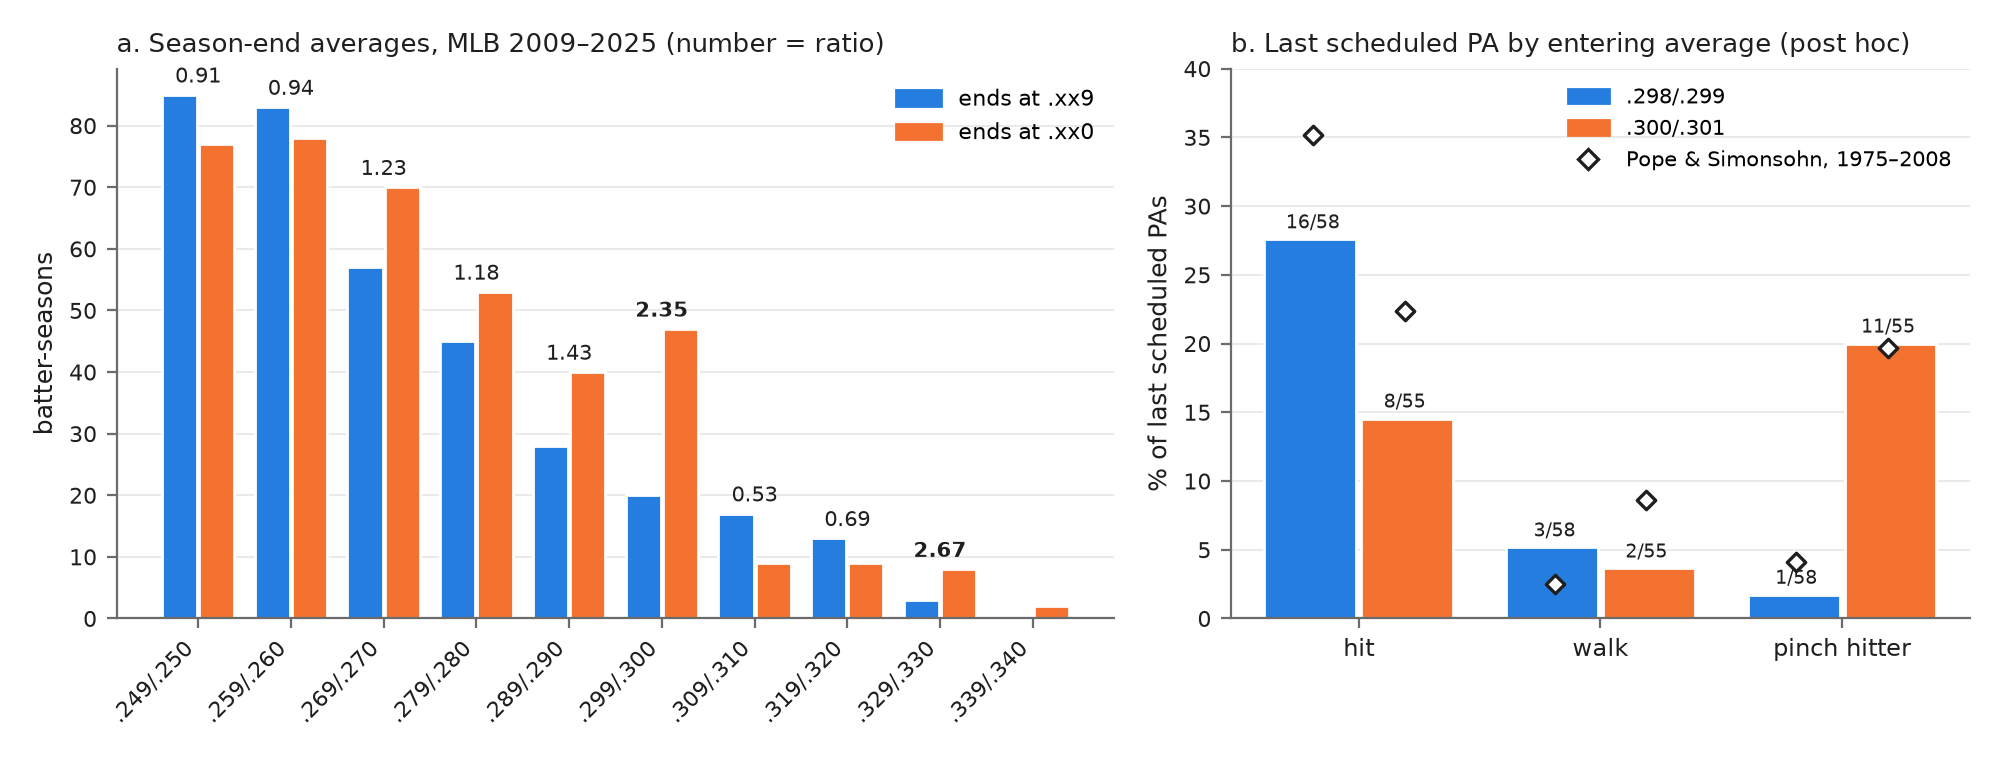
\includegraphics[width=\textwidth]{figures/fig1.png}
\caption{(a) Eligible batter-seasons that end just below (.xx9) and at (.xx0) each threshold, MLB 2009--2025; the number above each pair is the ratio $n_{x0}/n_{x9}$. The pair .349/.350 has no batter-season and is not drawn. (b) Outcome of the last scheduled PA by entering average (post hoc, exploratory), with the shares that Pope and Simonsohn report for 1975--2008 (diamonds). The labels give counts.}
\label{fig:main}
\end{figure}

\subsection{Season-end excess at .300 (T1, re-test)}

Of 5,447 eligible batter-seasons, 47 end at .300 (0.86\%) and 20 at .299 (0.37\%). The ratio is 2.35 (95\% Clopper--Pearson interval 1.37--4.19), and the one-sided binomial $p = 0.00065$. The original ratio, 1.40/0.38 = 3.7, is inside the interval. Table~\ref{tab:t1} and Figure~\ref{fig:main}a give the placebo thresholds. The ratio at .330 is 8/3 = 2.67, larger than at .300. By the registered rule, the claim is therefore \emph{not supported}, although the binomial test is significant. The counts above .320 are small, so a single placebo ratio can be large by chance; the rule was applied as written. The same counts follow from the official MLB totals alone (47 vs 20, 8 vs 3 at .330). In the paper's wider comparison (P1, post hoc), 44 seasons end at .298/.299 and 70 at .300/.301 (0.81\% vs 1.29\%; paper: 0.97\% vs 2.30\%), binomial $p = 0.0094$.

\begin{table}[t]
\centering
\caption{T1: eligible batter-seasons that end at .xx9 and at .xx0, MLB 2009--2025. The tenth placebo, .349/.350, has no batter-season (0 vs 0).}
\label{tab:t1}
\small\setlength{\tabcolsep}{4pt}
\begin{tabular}{lrrrrrrrrrr}
\toprule
Threshold & .250 & .260 & .270 & .280 & .290 & \textbf{.300} & .310 & .320 & .330 & .340 \\
\midrule
$n_{x9}$ & 85 & 83 & 57 & 45 & 28 & \textbf{20} & 17 & 13 & 3 & 0 \\
$n_{x0}$ & 77 & 78 & 70 & 53 & 40 & \textbf{47} & 9 & 9 & 8 & 2 \\
Ratio & 0.91 & 0.94 & 1.23 & 1.18 & 1.43 & \textbf{2.35} & 0.53 & 0.69 & 2.67 & -- \\
\bottomrule
\end{tabular}
\end{table}

\subsection{Last actual PA (T2, T3)}

Twenty-three eligible batters entered their last actual PA at .299. Three of them walked: Prince Fielder in 2009 and 2011, and Yainer Diaz in 2024. So the zero of the original sample does not persist. Against the original 0 of 61, the held-out 3 of 23 gives a two-sided Fisher $p = 0.019$; this comparison is descriptive. The walk share at .299 is 13.0\% (3/23), against 8.2\% (89/1,092) in LC. There is no walk suppression (T2, $p = 0.89$). In the same PA, .299 batters went 8 for 19 (.421) and .300 batters 4 for 20 (.200). The direction is the paper's, but the difference is not significant (T3, $p = 0.125$).

\subsection{Selection control (T4)}

In the team's last two games, group B (below .300, a hit reaches .300) went 62 for 217 (.286) and group A (at .300 or more, an out drops below .300) went 14 for 67 (.209). The difference has the paper's direction and is not significant ($p = 0.139$). The walk shares are 7.9\% (19/242) in B and 6.8\% (5/74) in A ($p = 0.70$). T3 is not significant, so the registered conditional statement about the Scott--Birnbaum account does not apply. The held-out data neither show a hit advantage below .300 nor exclude a small one.

\subsection{The paper's own comparisons (post hoc, exploratory)}

Table~\ref{tab:paper} and Figure~\ref{fig:main}b give P2--P6. The hit shares have the paper's direction and are not significant after the Holm correction. The P3 comparison group follows the paper's design and includes batters at .300; in that group, 30\% of the last scheduled PAs at .300 were substitutions, and a substitution cannot be a hit. So a part of the P3 gap can come from substitution. The walk shares are in the opposite direction to the paper. The substitution shares have the paper's direction and are significant after the Holm correction: 1.7\% (1/58) at .298/.299 against 20.0\% (11/55) at .300/.301, and 30.0\% (9/30) at .300 against 5.7\% (63/1,105) at the other values. These two results are post hoc and exploratory.

\begin{table}[t]
\centering
\caption{Last scheduled PA, the paper's comparisons (post hoc, exploratory). Shares include outs, hits, walks and substitutions in the denominator. Fisher $p$ is one-sided in the paper's direction, Holm-adjusted over P2--P6. ``Other'' is every value from .280 to .320 except the named one.}
\label{tab:paper}
\small\setlength{\tabcolsep}{3.5pt}
\begin{tabular}{llrrrr}
\toprule
 & Comparison & Paper 1975--2008 & 2009--2025 & Holm $p$ & $Z$ (two-sided $p$) \\
\midrule
P2 & hit, .298/.299 vs .300/.301 & 35.2\% vs 22.4\% & 16/58 vs 8/55 & 0.21 & 1.69 (0.090) \\
P3 & hit, .299 vs other & 43\% vs 22.8\% & 8/23 vs 229/1,112 & 0.21 & 1.66 (0.097) \\
P4 & walk, .298/.299 vs .300/.301 & 2.5\% vs 8.6\% & 3/58 vs 2/55 & 0.80 & 0.40 (0.69) \\
P5 & pinch hitter, .298/.299 vs .300/.301 & 4.1\% vs 19.7\% & 1/58 vs 11/55 & 0.006 & $-3.15$ (0.0016) \\
P6 & pinch hitter, .300 vs other & 34.3\% vs 7.0\% & 9/30 vs 63/1,105 & 0.0002 & 5.39 ($7\times10^{-8}$) \\
\bottomrule
\end{tabular}
\end{table}

\subsection{Exit check (descriptive)}

In the team's last three games, 105 eligible batters were at a displayed .300 after some PA. Of these, 38 (36.2\%) ended the season at .300. For the other values from .297 to .303 the share is 17.1\% to 26.1\%; all values are in \texttt{data/expected.json}. This check has no test. One batter can count at more than one value, so the groups overlap. The result is an association. It agrees with the selection account of Scott and Birnbaum and with the paper's own remark that batters at .300 end their season early. We did not test the cause: a manager, the batter, or the schedule can end a season.

\section{How the result was checked}
\label{sec:checks}

\paragraph{Validation of the parser.} \texttt{checks/rerun.py} downloads the MLB Stats API totals and compares hits and at-bats for every batter-season with at least 200 at-bats in either source. One of 5,447 differs: Luis Gonzalez (Retrosheet \texttt{gonzl005}), 2022, 79 hits in Retrosheet and 78 in the API, 311 at-bats in both. His average is about .254, so this cannot change a test. The cause is not known. Against Lahman (2009--2021), 0 of 4,082 batter-seasons differ. T1 computed from the MLB totals alone gives the same counts.

\paragraph{Independent recomputation.} A separate verification stage wrote its own parser with its own detection of rule 9.15(b) (86 reassignments, 2 Lahman mismatches). Its output reproduces every count of this paper: T1, L299, L300, LC, T4, the scheduled-PA groups and the three walkers. A second check counts T1 from the MLB Stats API totals only and recomputes every $p$-value, the interval and the Holm values from the counts. These scripts are in \texttt{checks/verify/}.

\paragraph{Rerun.} \texttt{bash checks/ci.sh} downloads about 133 MB of raw files, computes every number, and compares the full output with \texttt{data/expected.json}. On a clean copy it printed \texttt{MATCH expected.json} and exited 0. The run takes about 2 to 5 minutes, depending on the network and the machine. The SHA-256 values of the 17 Retrosheet files are stored in \texttt{expected.json}.

\paragraph{Prior art.} We searched two collections of AI-produced results and the AI result archives (terms ``Simonsohn'', ``round numbers'', ``.300 baseball'', ``pinch hitter''), Semantic Scholar citations of the paper (131 citing papers), and the web. We found the studies of Section 1 and no held-out test of the final-PA statements.

\section{Limits}

\begin{itemize}
\item Seventeen seasons give only 23 to 30 last PAs at .299 and at .300. The final-PA tests have low power. A non-significant result does not show that the effect is absent.
\item The registered walk and hit tests use press versions of the statements. The paper's own comparisons are tested post hoc only. The substitution result is exploratory and needs a test on new seasons.
\item The T1 placebo rule uses 10 thresholds with small counts above .320. It fails easily. We applied it as written.
\item The raw Retrosheet files were downloaded before the protocol commit. The record cannot show that no outcome was computed before it.
\item MLB corrects its records. A later download of the MLB Stats API can give a different validation count. The cause of the one mismatch is not known.
\item All results are associations. The data cannot tell whether a batter, a manager or chance ended a season at .300.
\end{itemize}

\section{Conclusion}

On 17 held-out seasons, more batters end the season at .300 than at .299, but the ratio is smaller than in 1975--2008 and the excess does not pass our pre-registered placebo rule. The statements that batters at .299 do not walk and get more hits in their last plate appearance do not replicate: walks occur, and the hit gap is not significant. A post hoc, exploratory analysis finds that batters at .300 are often replaced by a pinch hitter in their last scheduled plate appearance, as the paper reported. The post hoc substitution result and the descriptive exit check agree better with batters who stop at .300 than with batters who perform better below it. This is an association, not a test.

\begin{thebibliography}{99}
\bibitem{ps2011} D.~G. Pope and U.~Simonsohn. Round numbers as goals: evidence from baseball, SAT takers, and the lab. \emph{Psychological Science} 22(1):71--79, 2011. \url{https://doi.org/10.1177/0956797610391098}. Full text read from \url{https://web.archive.org/web/2012id_/http://opim.wharton.upenn.edu/~uws/papers/round_inpress.pdf}.
\bibitem{sb2010} P.~Scott and P.~Birnbaum. Do motivated players have higher batting averages? \emph{By the Numbers} (SABR Statistical Analysis Committee newsletter), February 2010. Web version 2011: \url{https://sabr.org/research/article/do-motivated-players-have-higher-batting-averages/}.
\bibitem{tanji2021} R.~Tanji. Reference dependence and monetary incentives: evidence from Major League Baseball. Discussion Paper 20-23, Graduate School of Economics, Osaka University, March 2021. \url{https://www2.econ.osaka-u.ac.jp/econ_society/dp/2023.pdf}.
\bibitem{nakamura2019} K.~Nakamura. Do round numbers always become reference points?: An examination by Japanese and Major League Baseball data. \emph{Proceedings of the Annual Meeting of the Cognitive Science Society} 41, 2019. \url{https://escholarship.org/uc/item/2c32h7gz}.
\bibitem{krab2023} H.~Krabbenhoft. Revisiting the psychology of ``round numbers as goals'': achieving a .300 batting average. Talk abstract in the SABR Baseball Records Committee newsletter, Summer 2023. \url{https://sabr.box.com/shared/static/7hra7d3yfo7dv2yhd0z2p7t798c6twk2.pdf}.
\bibitem{lombardi2011} S.~Lombardi. Prince Fielder's rare season ending walk. Baseball-Reference blog, 1 October 2011. \url{https://aws.baseball-reference.com/blog/archives/15489.html}.
\bibitem{retrosheet} Retrosheet. Regular-season event files 2009--2025. \url{https://www.retrosheet.org/events/}. Accessed 28 November 2026. The information used here was obtained free of charge from and is copyrighted by Retrosheet. Interested parties may contact Retrosheet at \url{https://www.retrosheet.org}.
\bibitem{mlbapi} MLB Advanced Media. MLB Stats API, season hitting totals. \url{https://statsapi.mlb.com/api/v1/stats}. Accessed 28 November 2026.
\bibitem{chadwick} Chadwick Baseball Bureau. Register of baseball persons. \url{https://github.com/chadwickbureau/register}, commit \texttt{ba48ce1}. Accessed 28 November 2026.
\bibitem{lahman} Chadwick Baseball Databank (Lahman database), \texttt{Batting.csv} and \texttt{People.csv}, mirror \url{https://github.com/cbwinslow/baseballdatabank}, commit \texttt{8a908d5}. Accessed 28 November 2026.
\end{thebibliography}

\end{document}
